%\subsection{Portfolio f\"ur Property Instance und Research Object (Gr\"o\ss{}e entspricht der Anzahl)}
%\begin{figure}
\begin{center}
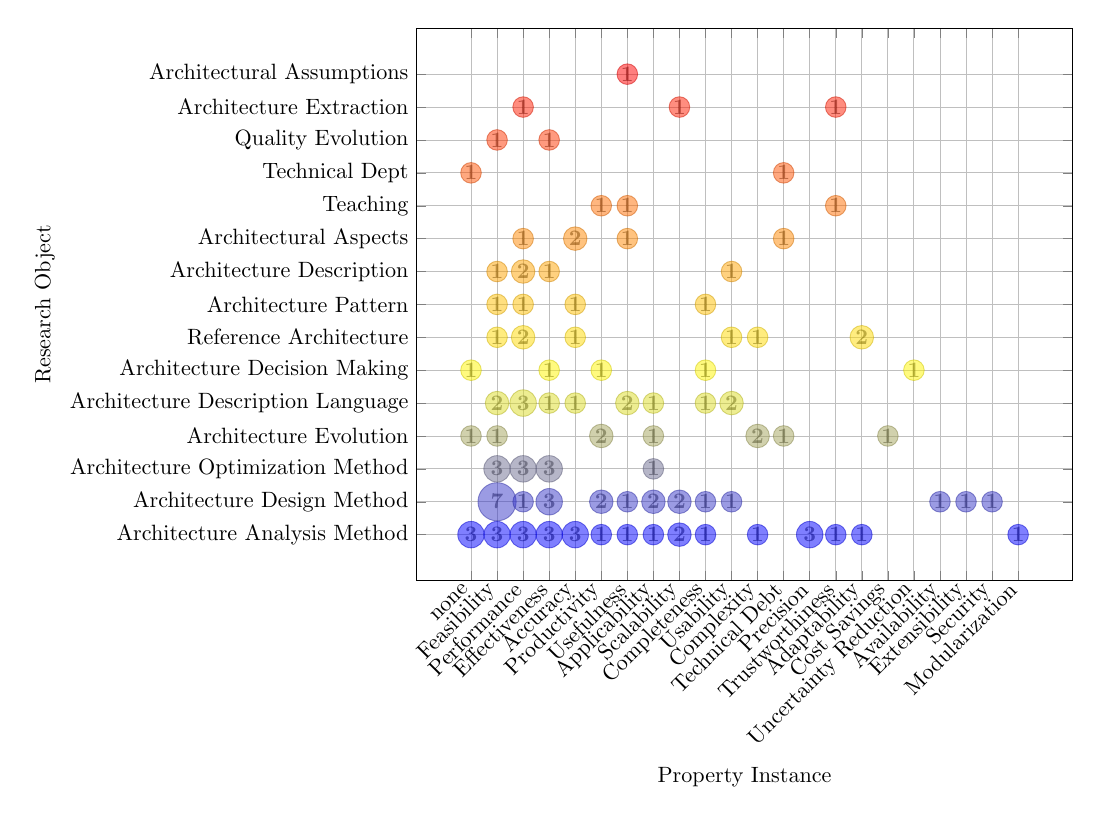
\begin{tikzpicture}[scale=.8]
\begin{axis}[scatter,
    width=.99\linewidth,
    cycle multi list=Spectral,
    every axis plot/.append style={draw, fill, fill opacity=0.5},
    scatter src=y,
    nodes near coords style={color=black,font=\small},
    %enlargelimits=0.15,
    x tick label style={rotate=45,anchor=east},
    xtick={0,1,2,3,4,5,6,7,8,9,10,11,12,13,14,15,16,17,18,19,20,21}, xticklabels={none,Feasibility,Performance,Effectiveness,Accuracy,Productivity,Usefulness,Applicability,Scalability,Completeness,Usability,Complexity,Technical Debt,Precision,Trustworthiness,Adaptability,Cost Savings,Uncertainty Reduction,Availability,Extensibility,Security,Modularization},
    xlabel={Property Instance},
    ytick={0,1,2,3,4,5,6,7,8,9,10,11,12,13,14}, yticklabels={Architecture Analysis Method,Architecture Design Method,Architecture Optimization Method,Architecture Evolution,Architecture Description Language,Architecture Decision Making,Reference Architecture,Architecture Pattern,Architecture Description,Architectural Aspects,Teaching,Technical Dept,Quality Evolution,Architecture Extraction,Architectural Assumptions},
    ylabel={Research Object},
    grid=both
]

\addplot[mark size=5.983,opacity=0.5,text=black] coordinates { (0,0) } node[text=black,font=\bfseries] {3};
\addplot[mark size=4.661,opacity=0.5,text=black] coordinates { (0,3) } node[text=black,font=\bfseries] {1};
\addplot[mark size=4.661,opacity=0.5,text=black] coordinates { (0,5) } node[text=black,font=\bfseries] {1};
\addplot[mark size=4.661,opacity=0.5,text=black] coordinates { (0,11) } node[text=black,font=\bfseries] {1};
\addplot[mark size=5.983,opacity=0.5,text=black] coordinates { (1,0) } node[text=black,font=\bfseries] {3};
\addplot[mark size=8.628,opacity=0.5,text=black] coordinates { (1,1) } node[text=black,font=\bfseries] {7};
\addplot[mark size=5.983,opacity=0.5,text=black] coordinates { (1,2) } node[text=black,font=\bfseries] {3};
\addplot[mark size=4.661,opacity=0.5,text=black] coordinates { (1,3) } node[text=black,font=\bfseries] {1};
\addplot[mark size=5.322,opacity=0.5,text=black] coordinates { (1,4) } node[text=black,font=\bfseries] {2};
\addplot[mark size=4.661,opacity=0.5,text=black] coordinates { (1,6) } node[text=black,font=\bfseries] {1};
\addplot[mark size=4.661,opacity=0.5,text=black] coordinates { (1,7) } node[text=black,font=\bfseries] {1};
\addplot[mark size=4.661,opacity=0.5,text=black] coordinates { (1,8) } node[text=black,font=\bfseries] {1};
\addplot[mark size=4.661,opacity=0.5,text=black] coordinates { (1,12) } node[text=black,font=\bfseries] {1};
\addplot[mark size=5.983,opacity=0.5,text=black] coordinates { (2,0) } node[text=black,font=\bfseries] {3};
\addplot[mark size=4.661,opacity=0.5,text=black] coordinates { (2,1) } node[text=black,font=\bfseries] {1};
\addplot[mark size=5.983,opacity=0.5,text=black] coordinates { (2,2) } node[text=black,font=\bfseries] {3};
\addplot[mark size=5.983,opacity=0.5,text=black] coordinates { (2,4) } node[text=black,font=\bfseries] {3};
\addplot[mark size=5.322,opacity=0.5,text=black] coordinates { (2,6) } node[text=black,font=\bfseries] {2};
\addplot[mark size=4.661,opacity=0.5,text=black] coordinates { (2,7) } node[text=black,font=\bfseries] {1};
\addplot[mark size=5.322,opacity=0.5,text=black] coordinates { (2,8) } node[text=black,font=\bfseries] {2};
\addplot[mark size=4.661,opacity=0.5,text=black] coordinates { (2,9) } node[text=black,font=\bfseries] {1};
\addplot[mark size=4.661,opacity=0.5,text=black] coordinates { (2,13) } node[text=black,font=\bfseries] {1};
\addplot[mark size=5.983,opacity=0.5,text=black] coordinates { (3,0) } node[text=black,font=\bfseries] {3};
\addplot[mark size=5.983,opacity=0.5,text=black] coordinates { (3,1) } node[text=black,font=\bfseries] {3};
\addplot[mark size=5.983,opacity=0.5,text=black] coordinates { (3,2) } node[text=black,font=\bfseries] {3};
\addplot[mark size=4.661,opacity=0.5,text=black] coordinates { (3,4) } node[text=black,font=\bfseries] {1};
\addplot[mark size=4.661,opacity=0.5,text=black] coordinates { (3,5) } node[text=black,font=\bfseries] {1};
\addplot[mark size=4.661,opacity=0.5,text=black] coordinates { (3,8) } node[text=black,font=\bfseries] {1};
\addplot[mark size=4.661,opacity=0.5,text=black] coordinates { (3,12) } node[text=black,font=\bfseries] {1};
\addplot[mark size=5.983,opacity=0.5,text=black] coordinates { (4,0) } node[text=black,font=\bfseries] {3};
\addplot[mark size=4.661,opacity=0.5,text=black] coordinates { (4,4) } node[text=black,font=\bfseries] {1};
\addplot[mark size=4.661,opacity=0.5,text=black] coordinates { (4,6) } node[text=black,font=\bfseries] {1};
\addplot[mark size=4.661,opacity=0.5,text=black] coordinates { (4,7) } node[text=black,font=\bfseries] {1};
\addplot[mark size=5.322,opacity=0.5,text=black] coordinates { (4,9) } node[text=black,font=\bfseries] {2};
\addplot[mark size=4.661,opacity=0.5,text=black] coordinates { (5,0) } node[text=black,font=\bfseries] {1};
\addplot[mark size=5.322,opacity=0.5,text=black] coordinates { (5,1) } node[text=black,font=\bfseries] {2};
\addplot[mark size=5.322,opacity=0.5,text=black] coordinates { (5,3) } node[text=black,font=\bfseries] {2};
\addplot[mark size=4.661,opacity=0.5,text=black] coordinates { (5,5) } node[text=black,font=\bfseries] {1};
\addplot[mark size=4.661,opacity=0.5,text=black] coordinates { (5,10) } node[text=black,font=\bfseries] {1};
\addplot[mark size=4.661,opacity=0.5,text=black] coordinates { (6,0) } node[text=black,font=\bfseries] {1};
\addplot[mark size=4.661,opacity=0.5,text=black] coordinates { (6,1) } node[text=black,font=\bfseries] {1};
\addplot[mark size=5.322,opacity=0.5,text=black] coordinates { (6,4) } node[text=black,font=\bfseries] {2};
\addplot[mark size=4.661,opacity=0.5,text=black] coordinates { (6,9) } node[text=black,font=\bfseries] {1};
\addplot[mark size=4.661,opacity=0.5,text=black] coordinates { (6,10) } node[text=black,font=\bfseries] {1};
\addplot[mark size=4.661,opacity=0.5,text=black] coordinates { (6,14) } node[text=black,font=\bfseries] {1};
\addplot[mark size=4.661,opacity=0.5,text=black] coordinates { (7,0) } node[text=black,font=\bfseries] {1};
\addplot[mark size=5.322,opacity=0.5,text=black] coordinates { (7,1) } node[text=black,font=\bfseries] {2};
\addplot[mark size=4.661,opacity=0.5,text=black] coordinates { (7,2) } node[text=black,font=\bfseries] {1};
\addplot[mark size=4.661,opacity=0.5,text=black] coordinates { (7,3) } node[text=black,font=\bfseries] {1};
\addplot[mark size=4.661,opacity=0.5,text=black] coordinates { (7,4) } node[text=black,font=\bfseries] {1};
\addplot[mark size=5.322,opacity=0.5,text=black] coordinates { (8,0) } node[text=black,font=\bfseries] {2};
\addplot[mark size=5.322,opacity=0.5,text=black] coordinates { (8,1) } node[text=black,font=\bfseries] {2};
\addplot[mark size=4.661,opacity=0.5,text=black] coordinates { (8,13) } node[text=black,font=\bfseries] {1};
\addplot[mark size=4.661,opacity=0.5,text=black] coordinates { (9,0) } node[text=black,font=\bfseries] {1};
\addplot[mark size=4.661,opacity=0.5,text=black] coordinates { (9,1) } node[text=black,font=\bfseries] {1};
\addplot[mark size=4.661,opacity=0.5,text=black] coordinates { (9,4) } node[text=black,font=\bfseries] {1};
\addplot[mark size=4.661,opacity=0.5,text=black] coordinates { (9,5) } node[text=black,font=\bfseries] {1};
\addplot[mark size=4.661,opacity=0.5,text=black] coordinates { (9,7) } node[text=black,font=\bfseries] {1};
\addplot[mark size=4.661,opacity=0.5,text=black] coordinates { (10,1) } node[text=black,font=\bfseries] {1};
\addplot[mark size=5.322,opacity=0.5,text=black] coordinates { (10,4) } node[text=black,font=\bfseries] {2};
\addplot[mark size=4.661,opacity=0.5,text=black] coordinates { (10,6) } node[text=black,font=\bfseries] {1};
\addplot[mark size=4.661,opacity=0.5,text=black] coordinates { (10,8) } node[text=black,font=\bfseries] {1};
\addplot[mark size=4.661,opacity=0.5,text=black] coordinates { (11,0) } node[text=black,font=\bfseries] {1};
\addplot[mark size=5.322,opacity=0.5,text=black] coordinates { (11,3) } node[text=black,font=\bfseries] {2};
\addplot[mark size=4.661,opacity=0.5,text=black] coordinates { (11,6) } node[text=black,font=\bfseries] {1};
\addplot[mark size=4.661,opacity=0.5,text=black] coordinates { (12,3) } node[text=black,font=\bfseries] {1};
\addplot[mark size=4.661,opacity=0.5,text=black] coordinates { (12,9) } node[text=black,font=\bfseries] {1};
\addplot[mark size=4.661,opacity=0.5,text=black] coordinates { (12,11) } node[text=black,font=\bfseries] {1};
\addplot[mark size=5.983,opacity=0.5,text=black] coordinates { (13,0) } node[text=black,font=\bfseries] {3};
\addplot[mark size=4.661,opacity=0.5,text=black] coordinates { (14,0) } node[text=black,font=\bfseries] {1};
\addplot[mark size=4.661,opacity=0.5,text=black] coordinates { (14,10) } node[text=black,font=\bfseries] {1};
\addplot[mark size=4.661,opacity=0.5,text=black] coordinates { (14,13) } node[text=black,font=\bfseries] {1};
\addplot[mark size=4.661,opacity=0.5,text=black] coordinates { (15,0) } node[text=black,font=\bfseries] {1};
\addplot[mark size=5.322,opacity=0.5,text=black] coordinates { (15,6) } node[text=black,font=\bfseries] {2};
\addplot[mark size=4.661,opacity=0.5,text=black] coordinates { (16,3) } node[text=black,font=\bfseries] {1};
\addplot[mark size=4.661,opacity=0.5,text=black] coordinates { (17,5) } node[text=black,font=\bfseries] {1};
\addplot[mark size=4.661,opacity=0.5,text=black] coordinates { (18,1) } node[text=black,font=\bfseries] {1};
\addplot[mark size=4.661,opacity=0.5,text=black] coordinates { (19,1) } node[text=black,font=\bfseries] {1};
\addplot[mark size=4.661,opacity=0.5,text=black] coordinates { (20,1) } node[text=black,font=\bfseries] {1};
\addplot[mark size=4.661,opacity=0.5,text=black] coordinates { (21,0) } node[text=black,font=\bfseries] {1};


\end{axis}
\end{tikzpicture}
\end{center}
%\caption{Portfolio f\"ur Property Instance und Research Object (Gr\"o\ss{}e entspricht der Anzahl)}\label{fig:port_propertyinstance_researchobject}
%\end{figure}

